\chapter{Introduction}
While approaching a more and more ubiquitous network experience where we are
connected to different personal area networks (PAN) or even the global internet
around the clock two problems become more important. One problem is the power
consumption of devices which make the ubiquity possible. In contrast to other
computing devices we want them to be well hidden and unintrusive. Changing
batteries or having power cables around is not a real option for them. On the
other hand wireless communication protocols with IEEE 802.11 \cite{ieee80211} as the
leading option are a good choice for mobile devices like notebooks or
smartphones but are still to power hungry for small ubiquitous devices.
With IEEE 802.15.4 \cite{ieee802154} a new protocol was designed for exactly such
small, power constraint devices. We will use it in our research and have some
more information about it prepared in section~\ref{intro802154}.

The second problem are network connection disruptions - be it due to movement or
the other changes. The most widely used protocol family with IP, UDP, TCP is not
designed to cope with disrupted networks. They need a (mostly) working physical connection
to work as expected. If this is not the case the packets may be just lost
as in case of UDP or have to be re-transmitted. This re-transmission could be
problematic if the network connection is unavailable more often then available.
For such scenarios delay tolerant networking was designed to send the
packets, perhaps over several hops, to the destination without needing to
establish a channel between source and destination. In~\ref{introdtn} we give a
short introduction to DTN before describing the IBR-DTN implementation in chapter
\ref{ibr-dtn} and our convergence layer in chapter \ref{802154layer}.

\section{IEEE 802.15.4}
\label{intro802154}
Driven by an IEEE working group the IEEE 802.15.4 standard provides the physical and
media access control layer for so called low-rate wireless personal area network
(LR-WPAN). The emphasis is on low cost devices for communication without
infrastructure over small distances. The communication range would be up to
10m and offers a transfer rate up to 250 kbps. The standard specifies
three possible frequency bands to operate in. The usage of some may be
restricted in different countries but one band is available worldwide. Other
features of IEEE 802.15.4 includes collision avoidance through CSMA/CA, built in
support for secure communication through cryptography, power management through
link quality control and energy detection as well as reserved time slots for
real-time operations.

As already described the standard only covers the two lowest layer of a
protocol stack. Supplementing it to a fully functional networking stack is the aim
of different other specifications as shown in figure~\ref{fig:802154layer}. The
most widely know is be ZigBee. With 6LowPAN there is also work underway to combine
LR-WPAN with standard internet protocols like IPv6.

Specified for an infrastructure-less network the topologies may be star or
Peer-to-Peer based as well a combination of both. Figure \ref{fig:802154topologies}
shows how an example star network topology could look as well as a Peer-to-Peer
topology. Two different device types are allowed: full-function device (FFD) and
reduced-function device (RFD). The RFD is a very simple device which can only
connect to one FFD at a time. Therefore it can only act as a leaf in all
described topologies. In contrast the FFD is able to act as a coordinator to
create a new PAN and relay messages to other nodes. At least one coordinator
is needed in every network. One thing to keep in mind is that routing is not
covered by the standard. To relay messages over multiple hops the supplementing
upper layers need to take care of this.

\begin{figure}
  \begin{center}
    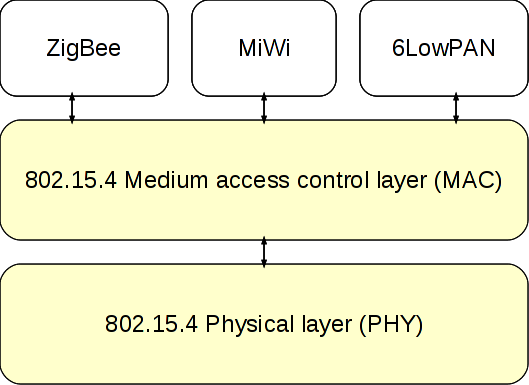
\includegraphics[height=6cm]{images/802154layer}
    \caption{IEEE 802.15.4 lower layers with optional upper layers}
        \label{fig:802154layer}
  \end{center}
\end{figure}

\begin{figure}
  \begin{center}
    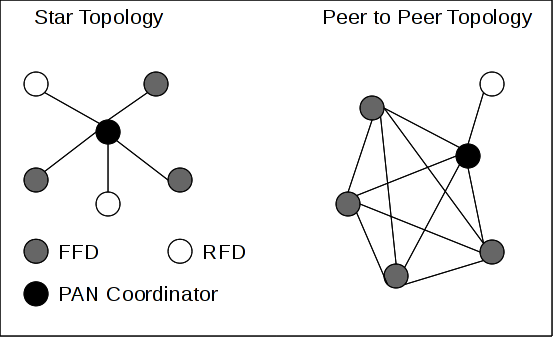
\includegraphics[height=6cm]{images/802154topology}
    \caption{IEEE 802.15.4 network topologies}
        \label{fig:802154topologies}
  \end{center}
\end{figure}

\section{DTN}
\label{introdtn}
Delay-tolerant networking is the other core technology that is used within this
thesis. The need for communication between nodes without continuous network
connectivity is what DTN seeks to address. Most modern routing protocols only
send out the payload once a complete route to the destination has been established.
A communication over such an approach is only possible if source and destination
are connected to a network long enough to establish a route between them,
transfer the data and possibly acknowledge the transfer.

DTN in contrast uses a store and forward approach which sends out the data
together with the destination address. The bundle protocol in
\cite{RFC5050} was specified for this. One approach to maximize the probability
of a successful delivered message would be to send out multiple copies of the
same message, maybe to different hops. Such an approach obviously increases the
network and storage load and may not be useful for constrained devices like
sensor nodes.

The bundle protocol specifies an overlay network which interacts with the lower
layers over convergence layers. The lower layers are not bound to be IP
based even if that is the one widely used. In this thesis we describe the usage
of the DTN implementation IBR-DTN over an IEEE 802.15.4 radio link on a Linux
based system.
